

%%%%%%%%%%%%%%%%%%%%%%%%%%%%%%%%%%%%%%%%%
% University/School Laboratory Report
% LaTeX Template
% Version 3.1 (25/3/14)
%
% This template has been downloaded from:
% http://www.LaTeXTemplates.com
%
% Original author:
% Linux and Unix Users Group at Virginia Tech Wiki 
% (https://vtluug.org/wiki/Example_LaTeX_chem_lab_report)
%
% License:
% CC BY-NC-SA 3.0 (http://creativecommons.org/licenses/by-nc-sa/3.0/)
%
%%%%%%%%%%%%%%%%%%%%%%%%%%%%%%%%%%%%%%%%%

%----------------------------------------------------------------------------------------
%	PACKAGES AND DOCUMENT CONFIGURATIONS
%----------------------------------------------------------------------------------------

\documentclass{article}

\usepackage[version=3]{mhchem} % Package for chemical equation typesetting
\usepackage{siunitx} % Provides the \SI{}{} and \si{} command for typesetting SI units
\usepackage{graphicx} % Required for the inclusion of images
\usepackage{natbib} % Required to change bibliography style to APA
\usepackage{amsmath} % Required for some math elements 
\usepackage{listings}
\usepackage{color}
\usepackage{caption}

\definecolor{dkgreen}{rgb}{0,0.6,0}
\definecolor{gray}{rgb}{0.5,0.5,0.5}
\definecolor{mauve}{rgb}{0.58,0,0.82}

\lstset{frame=tb,
  language=Java,
  aboveskip=3mm,
  belowskip=3mm,
  showstringspaces=false,
  columns=flexible,
  basicstyle={\small\ttfamily},
  numbers=none,
  numberstyle=\tiny\color{gray},
  keywordstyle=\color{blue},
  commentstyle=\color{dkgreen},
  stringstyle=\color{mauve},
  breaklines=true,
  breakatwhitespace=true,
  tabsize=3
}
\setlength\parindent{0pt} % Removes all indentation from paragraphs

\renewcommand{\labelenumi}{\alph{enumi}.} % Make numbering in the enumerate environment by letter rather than number (e.g. section 6)

%\usepackage{times} % Uncomment to use the Times New Roman font

%----------------------------------------------------s------------------------------------
%	DOCUMENT INFORMATION
%----------------------------------------------------------------------------------------

\title{Laboratory Assignment 1 Write Up \\ Computer Science 441} % Title

\author{\textsc{Andreas Bach Landgrebe} \\} % Author name

\date{\today} % Date for the report

\begin{document}

\maketitle % Insert the title, author and date

\begin{center}
\begin{tabular}{l r}
Date Submitted:  February 8, 2016 \\ % Date the experiment was performed
Partners:  Andreas Bach Landgrebe  \\ % Partner names
Instructor:  Dr. Gregory M. Kapfhammer  % Instructor/supervisor
\end{tabular}
\end{center}

% If you wish to include an abstract, uncomment the lines below
% \begin{abstract}
% Abstract text
% \end{abstract}

%----------------------------------------------------------------------------------------
%	SECTION 1
%----------------------------------------------------------------------------------------

\section{The commented source code of the Java classes that perform client-server-based file transfer.}

FileSocketClient.java
\begin{lstlisting}
import java.io.DataOutputStream;
import java.io.FileInputStream;
import java.io.IOException;
import java.net.Socket;
import java.io.File;
import java.util.ArrayList;
import java.util.List;

// This class is based off of the example at:
// https://gist.github.com/CarlEkerot/2693246

public class FileSocketClient {

    private Socket s;

    public FileSocketClient(String host, int port, String file) {
        //this is the constructor.
        //the host is a device with an IP address.
        //an IP address is a unique number to identify a number.
        //an port is a way to organize programs since different programs listen to different ports.
        //In this case, these programs interact at port 12345. 

        try {
            //try to connect to the server
            s = new Socket(host, port);
            sendFile(file);
        } catch (Exception e) {
            e.printStackTrace();
        }
    }

    public void sendFile(String file) throws IOException {
        File sendFile = new File(file);
        Long sendFileSize;
        DataOutputStream dos = new DataOutputStream(s.getOutputStream()); //this is the data the client is sending as output
        FileInputStream fis = new FileInputStream(file); //This is the file that the server is taking as input
        String sendFileName = sendFile.getName();
        sendFileSize = sendFile.length();

        byte[] buffer = new byte[4096];
        //the amount of bytes being read each time so the the file is being read in pieces instead of the whole thing

        dos.writeLong(sendFileSize);
        dos.writeUTF(sendFileName);

        while (fis.read(buffer) > 0) { //if the data output stream has been read server from the server, then write to it.
            dos.write(buffer); //write to the file input stream
        }
        //close the data output stream and file input stream like a good boy
        fis.close();
        dos.close();
    }

    public static void main(String[] args) {
        int i=0;
        String hostName = "localhost"; //default name for hostName
        int portNumber = 12345; //default port number
        ArrayList<String> fileNames = new ArrayList<String>();
        //arraylist used to store the filesNames that is being sent to the server
        while (i<args.length) {
            if ((args[i]=="-host") || (args[i]=="-h")) { 
                hostName = args[++i]; //if -host or -h is specified, then the next argument is the host name
            } 
            else if ((args[i]=="-port") || (args[i]=="-p")) {
                portNumber = Integer.parseInt(args[++i]);
                //if -port or -p is specified, then the next argument is the port number
            } else {
                fileNames.add(args[i]); //else it is assumed to be a file name
            }
            i++;

        }

        for (i=0; i<fileNames.size();i++) {
           FileSocketClient fc = new FileSocketClient(hostName, portNumber, fileNames.get(i)); 
           //for loop to transfer all of the files and arguments          
        }

        //FileSocketClient fc = new FileSocketClient("localhost", 12345, "files/send/seke2015-kinneer-kapfhammer-wright-mcminn.pdf");
          //FileSocketClient fc = new FileSocketClient(args[0], Integer.parseInt(args[1]), args[2]);
          //args[0] is the host so "localhost"
          //args[1] is the port so 12345
          //args[2] is the fileName

    }

}

\end{lstlisting}

FileSocketServer.java
\begin{lstlisting}
import java.io.DataInputStream;
import java.io.FileOutputStream;
import java.io.IOException;
import java.net.ServerSocket;
import java.net.Socket;
import java.text.DecimalFormat;

// This class is based off of the example at:
// https://gist.github.com/CarlEkerot/2693246

public class FileSocketServer extends Thread {

    private ServerSocket ss;

    public FileSocketServer(int port) {
        try {
            ss = new ServerSocket(port);
        } catch (IOException e) {
            e.printStackTrace();
        }
    }

    public void run() {
        while (true) {
            try {
                Socket clientSock = ss.accept();
//The accept method waits until a client starts up and requests a connection on the host and port of this server.
//Since it is a thread we are working with, it will run in parallel with other processes or threads in this multi-threaded system.

                saveFile(clientSock);
                //this method call will save the file
            } catch (IOException e) {
                e.printStackTrace();
            }
        }
    }

    private void saveFile(Socket clientSock) throws IOException {
        DataInputStream dis = new DataInputStream(clientSock.getInputStream());

        long fSize; //long variable for the size of the file
        String fName; //string variable for the name of the file
		
	   long startTime = System.currentTimeMillis();	   
	   
        fSize = dis.readLong(); //having the server read the size of the file
        fName = dis.readUTF(); //having the server read the name of the file

        FileOutputStream fos = new FileOutputStream("files/received/" + fName); 
        //this is the locations where the file that is going through the client server interfaction will end up
        //the paper will be remained paper.pdf.
        byte[] buffer = new byte[4096];
        //this is the amount of bytes being used to read the file as pieces instead of reading the entire file at once
        int filesize =  (int) fSize; //401210; // Send the file size in a separate message, hard-coded for right now
        int read = 0;
        int totalRead = 0;
        int remaining = filesize;
        while((read = dis.read(buffer, 0, Math.min(buffer.length, remaining))) > 0) {
            totalRead += read;
            remaining -= read;
            System.out.println("read " + totalRead + " bytes.");
            fos.write(buffer, 0, read); //
        }
        long stopTime = System.currentTimeMillis();
        long elapsedTime = stopTime - startTime;
        DecimalFormat df = new DecimalFormat ("#0.0000");
        System.out.println(df.format(elapsedTime));
        //close the data input stream and file output stream like a good boy
        fos.close(); //close the data input stream
        dis.close(); //close the file output stream
    }

    public static void main(String[] args) {
        FileSocketServer fs = new FileSocketServer(12345);
        fs.start(); //start the file socket server using the port 12345.
    }

}

\end{lstlisting}
%----------------------------------------------------------------------------------------
%	SECTION 2
%----------------------------------------------------------------------------------------

\section{Using both text and diagrams, a description of client-server-based file transfer with sockets.}
To best provide a description of client-served-based file transfer with sockets, the below figure illustrates the relationship between the client/server of the sockets \cite{ibm_knowledge_center}
\begin{center}
\vspace{-10em}
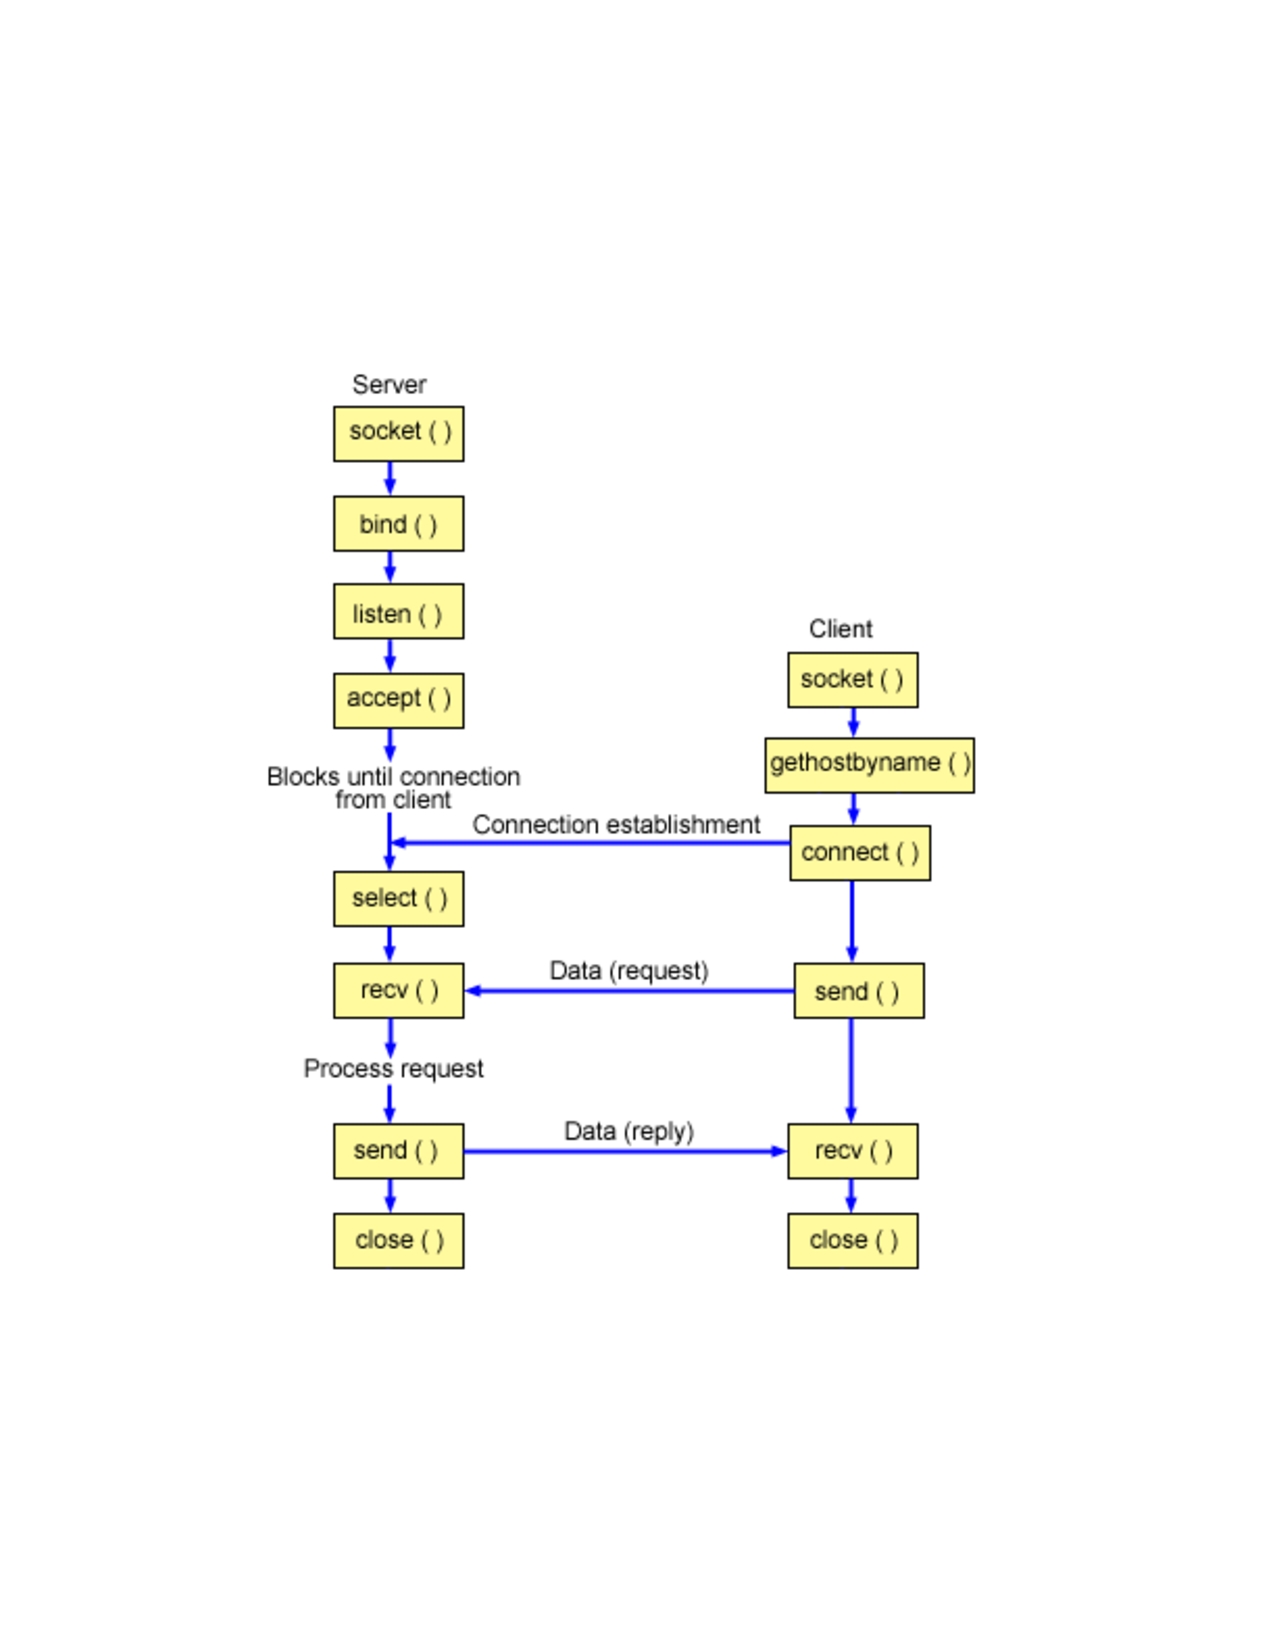
\includegraphics[scale=0.5]{CSsockets.pdf}
\vspace{-10em}
\end{center}
In this diagram, the first event that occurs is that the socket() method will return a socket descriptor wich represents an endpoint \cite{ibm_knowledge_center}.
After this, still being on the the server, the bind() method will get a unique name for the socket \cite{ibm_knowledge_center}. Then, the listen() method will listen for incoming connections buy the client. After it listen, the accept() method will accept incoming connections from the client. After the connection has been established, the select() method will allow the process to wait for an event to occur \cite{ibm_knowledge_center}. After an event has occurred which includes having the server request data from the client, the server will receive the information in the recv() method. The server will then process the request and have the send() method send data back as a reply. After the data has been replied, the connection from the client to the server will be closed.
In terms of the client, the socket() method will reutrn a socket descsiptor, which represents an endpooint \cite{ibm_knowledge_center}. After the socket() method, the gethostbyname() will get the IP address of the server. Once the client has got the IP address of the server, the connect() method will connect to the server. Once the connection has been established, the client will then go to the send() method where the client will request data from the server. Once the server receives the call, the server will reply back and the client will receive the data through the recv() method. Once the data is received from the server, the connection between the client and the server will be closed through the close() method. 

%----------------------------------------------------------------------------------------
%	SECTION 3
%----------------------------------------------------------------------------------------
\section{A description of the challenges associated with performing client-server communication.}

There can quite a few challenges assocaited with performing client-server communication. One of the these challenges may include having a issue with the use of which port. The purpose of a port is to be able to organize accordingly since different programs and pieces of software use different ports to interact with one another. If a port is already in use for different purpose, the communication between the client and server may conflict with one another. The main challenge around this issue is organize ports accordingly so there are no conflictions. Another challenge that arises when thinking about performing client-server communication is thinking in terms of client that requests services from servers that helps us understand and manage the complexity of distributed systems \cite{tanenbaum_steen_2007}.
%----------------------------------------------------------------------------------------
%	SECTION 4
%----------------------------------------------------------------------------------------

\section{A comparison of file transfer methods that use ``centralized" and ``decentralized" approaches}

There are two different approaches being discussed throughout the book when looking at file transfer methods. The first one that is being looked at is a centralized architecture approach. In a centralized approach, there is a general interaction between a client and server. The below diagram displays what the interaction looks like between a client and a server.
\begin{center}
\vspace{-10em}
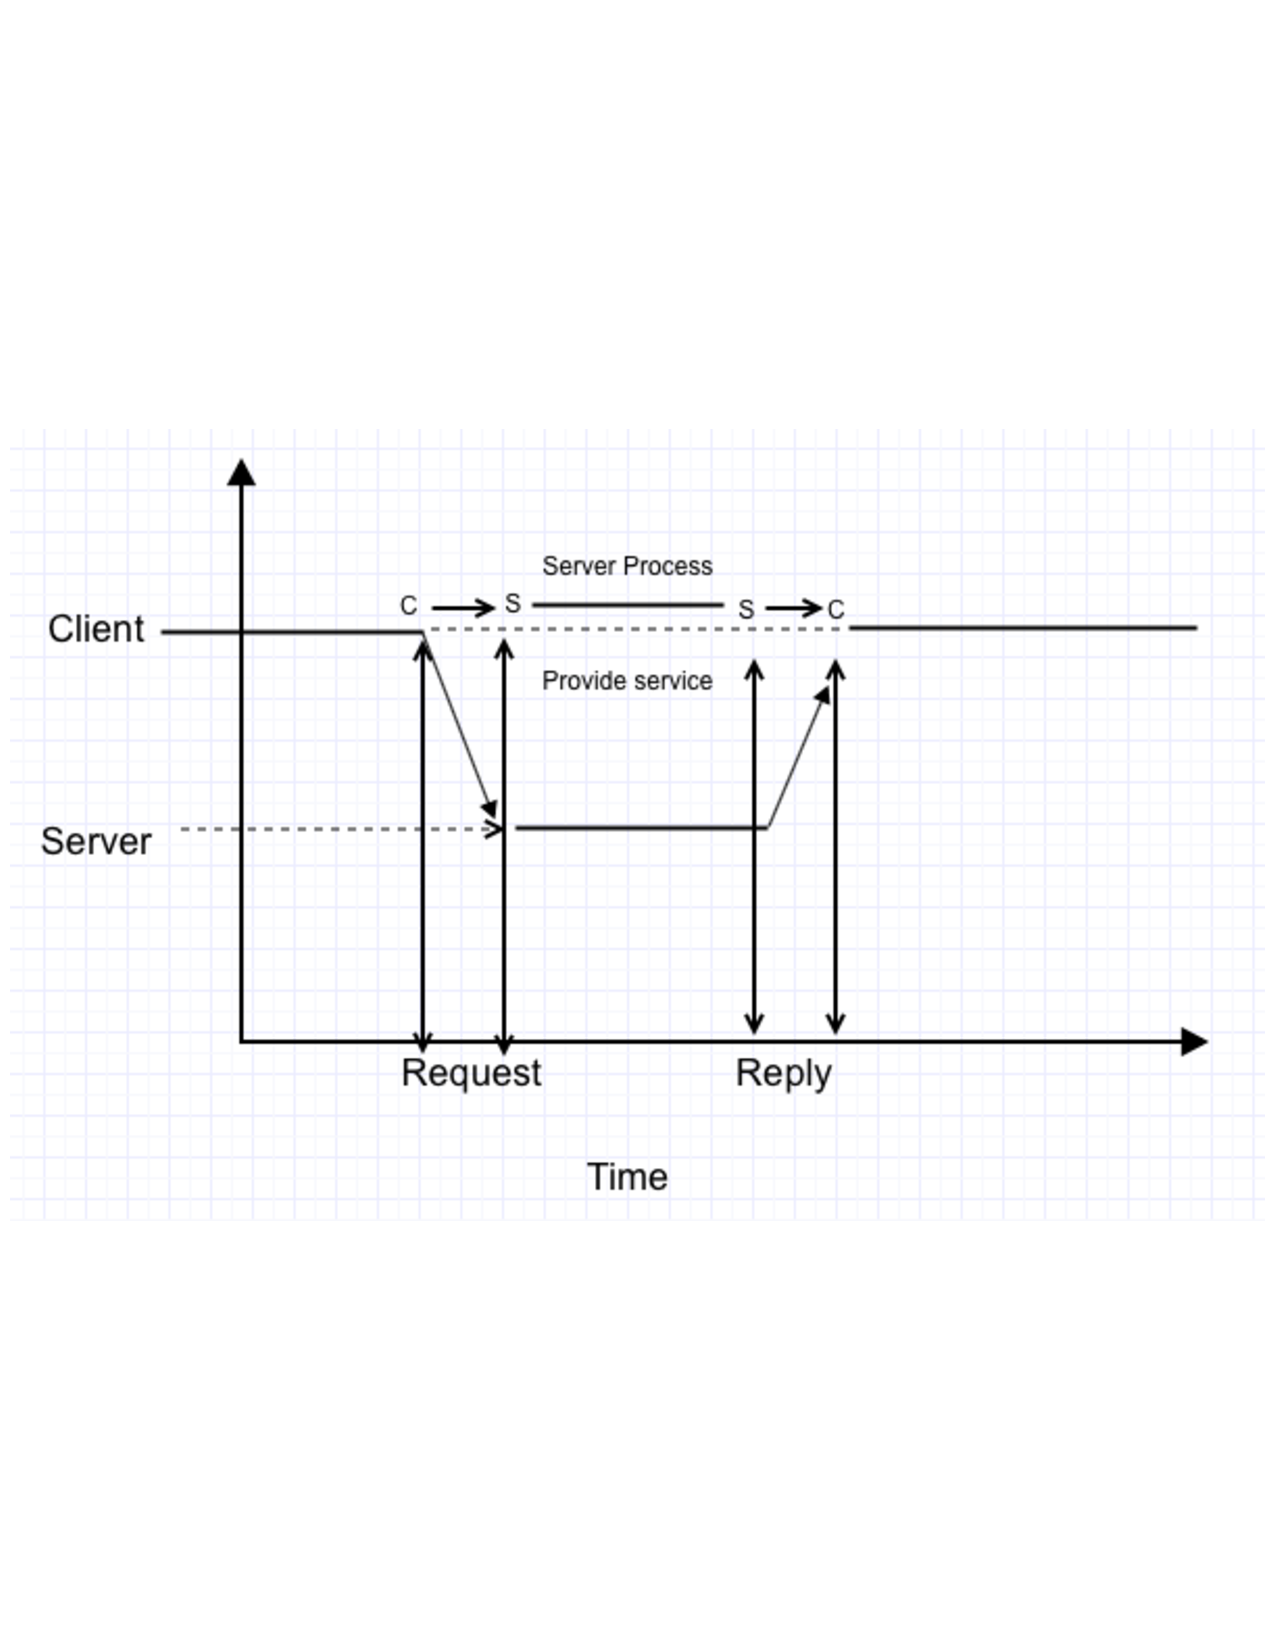
\includegraphics[scale=0.5]{Centralized.pdf}
\vspace{-10em}
\end{center}
The above diagram illustrates the general interaction between the client and the server. This figure was layed out on page 37 of the Distributyed Systems book by Andrew Tannebaum and Maarten Van Steen \cite{tanenbaum_steen_2007}. In this diagram, the first event that occurs is the client requesting from the server. In the diagram, the C stands for Client and the S stans for Server. After the Request has been undergone, then the Server Process is undergone. Another way of saying this is to provide a service or the response time of the server. After the server process has been completed, then the server will reply top the client. This is the idea of a general interaction between a client and a server throughout a centralized approach.
\par
%Talk about the Decentrlaized Approach Here
Now, there is another approach that can be used to conduct file transfer methods. This method is know as decentralized methods. One key idea behind this architecture is the idea of a distribution called vertical distribution. In vertical distribution, different compponenet are placed logically on different machines. This term is also related to the concept of veritcal fragmentation. This means that table are distributed across multiple machines \cite{tanenbaum_steen_2007}. The biggest difference between these two approaches is that centralized architecture include having one ``centralized" computer to act as a server and in a ``decentralized" approach, infomration has a distribution across multiple machines. 


%----------------------------------------------------------------------------------------
%	SECTION 5
%----------------------------------------------------------------------------------------
\section{A detailed paper that reports on the empirical results arising from performing file transfers.}

When completing the assignment, I have set up a few argument variables. Some of these include the host. If one writes -host, then the following argument will have to be the localhost. In these case, it would be the localhost. I have also set up the port. If one writes -port, then the following will includ eto specificy a port number. For the purposes of this laboratory assignment, it would be 12345. The next variable set up will be an arrayList called fileNames. This arrayList is used to store to names of the file names that is being sent to the server. The files being sent to the server includes kapfhammerSmall.pdf, KKWMmedium.pdf, and textbookLarge.pdf. These pdf files are included in the version control repository that I have shared. The kapfhammerSmall.pdf files is 239 KB. The KKWMmedium.pdf is 401 KB. The textbookLarge is 10 MB. These 3 files are being used as my "small", "medium", and "large"
files sizes when using the FileSocketClient and FileSocketServer.     
\par
For the small pdf file, here are the results
\begin{lstlisting}
kapfhammerSmall.pdf
1: 8.0000 ms
2: 8.0000 ms
3: 4.0000 ms
4: 10.0000 ms
5: 5.0000 ms
6: 5.0000 ms
7: 13.0000 ms
8: 5.0000 ms
9: 4.0000 ms
10: 5.0000 ms
Mean (Average): 6.7
Standard Deviation: 2.98329
\end{lstlisting}
For the medium pdf file, here are the results
\begin{lstlisting}
KKWMmediumpdf
1: 38.0000 ms
2: 9.0000 ms
3: 5.0000 ms
4: 6.0000 ms
5: 6.0000 ms
6: 5.0000 ms
7: 10.0000 ms
8: 5.0000 ms
9: 6.0000 ms
10: 4.0000 ms
Mean: 9.4
Standard Deviation: 10.22198
\end{lstlisting}

For the large pdf file, here are the results
\begin{lstlisting}
textbookLarge.pdf
1: 911.0000 ms
2: 22.0000 ms
3: 56.0000 ms
4: 32.0000 ms
5: 21.0000 ms
6: 39.0000 ms
7: 26.0000 ms
8: 21.0000 ms
9: 21.0000 ms
10: 19.0000 ms
Mean: 116.8
Standard Deviation: 279.2895
\end{lstlisting}
%-----------------------------------------------
%	SECTION 6
%-----------------------------------------------
\section{A description of the challenges that you encountered when completing this assignment.}

There were a few challenges that I have encountered when completing this assignment. One of these challenges included specifying the size of the file in the FileSocketClient.java file. This arose an issue due to the fact that the args[] variable that I was using included specifying the host, port, and file in the client side. Thankfull, I was able to overcome this challenge. Another challenge that came up throughout the completing of this laboratory assignment was understanding the byte[] buffer declaration. In this declaration, this variable specifies the number of bytes being used to read in the file. The challenge behind this was understand the file was being read in as pieces compared to reading the whole file at once.


%----------------------------------------------------------------------------------------
%	BIBLIOGRAPHY
%----------------------------------------------------------------------------------------

\nocite{ibm_knowledge_center}
\nocite{www.tutorialspoint.com}

\bibliographystyle{plain}

\bibliography{sample}

%----------------------------------------------------------------------------------------


\end{document}
